\documentclass[letterpaper,11pt,twoside]{article}
\usepackage[margin=0.88in]{geometry}

%%%%%%%%%%%%%%%%%%%%%%%%%%%%%%%%%%%%%%%%%%%%%%%%%%%%%%%%%%%%%%%%%%%%%%%%%%%%%%%


\def\mypdfauthor{Dimitris Diochnos}
\def\mypdfsubject{Undergraduate Course}
\def\mypdftitle{CS 3823 - Theory of Computation, 2025F: HW2}
\def\myheadertitle{CS 3823 - Theory of Computation: Homework Assignment 2}
\def\mytitle{CS 3823 - Theory of Computation: Homework Assignment 2}
\def\thecurrentsemester{Fall 2025}
\def\myduedate{\textbf{Due:} Friday, October 3, 2025}

%%%%%%%%%%%%%%%%%%%%%%%%%%%%%%%%%%%%%%%%%%%%%%%%%%%%%%%%%%%%%%%%%%%%%%%%%%%%%%%
\usepackage{xspace}
\usepackage{enumitem}
%\usepackage[numbers,square,sectionbib,sort&compress]{natbib}
\usepackage[numbers,square,sort&compress]{natbib}
\usepackage[euler-digits, T1]{eulervm}
\usepackage{upgreek}
\usepackage[dvipsnames]{xcolor}
\usepackage[
   colorlinks%
   ,plainpages=false%This forces a unique identification of pages.
   ,hypertexnames=true%This is necessary to have exact link on Index page.
   ,naturalnames
   ,hyperindex
   ,citecolor=OliveGreen
   ,urlcolor=RoyalBlue
   ,pdfauthor={\mypdfauthor}
   ,pdftitle={\mypdftitle}
   ,pdfsubject={\mypdfsubject}
   %,pdfkeywords={...}
]{hyperref}
%\usepackage{lettrine}
%\input{definitions}
\usepackage{psfrag}
\usepackage{graphicx}
\usepackage{multirow}
\usepackage{multicol}
\usepackage{array}
%\usepackage{vwcol}
\usepackage{enumitem}

%%%%%%%%%%%%%%%%%%%%%%%%%%%%%%%%%%%%%%%%%%%%%%%%%%%%%%%%%%%%%%%%%%%

\usepackage{bm}
\usepackage{pstricks}
\psset{unit=0.45cm}
\psset{linewidth=0.05}%
\psset{fillstyle=solid}%

\newcommand{\sample}{\ensuremath{S}\xspace}
\newcommand{\XX}{\ensuremath{\mathcal{X}}\xspace} % X

%%%%%%%%%%%%%%%%%%%%%%%%%%%%%%%%%%%%%%%%%%%%%%%%%%%%%%%%%%%%%%%%%%%

\usepackage{fancyhdr}
\pagestyle{fancy}
\usepackage{lastpage}
\usepackage{tikz}

\setlength{\headheight}{14pt}

\fancypagestyle{firststyle}
{
   \fancyhf{}
   \fancyfoot[L]{\today}
   %\fancyfoot[C]{\thepage/\pageref*{LastPage}}
   \fancyfoot[R]{\thepage/\pageref*{LastPage}}
}


\newcommand{\stylishPagesColor}{Gray}
\newcommand{\stylishHref}[2]%
{\hypersetup{urlcolor=\stylishPagesColor}%
\href{#1}{#2}%
\hypersetup{urlcolor=RoyalBlue}}


\fancyhead{} % clear all header fields
\fancyhead[CO,CE]{\textsc{\myheadertitle}}
\fancyfoot{} % clear all footer fields
\fancyfoot[LO,RE]{\today}
\fancyfoot[RO,LE]{\thepage/\pageref*{LastPage}}
\renewcommand{\headrulewidth}{0.0pt}
\renewcommand{\footrulewidth}{0.0pt}
%%%%%%%%%%%%%%%%%%%%%%%%%%%%%%%%%%%%%%%%%%%%%%%%%%%%%%%%%%%%%%%%%%%
\newcommand{\OO}[1]{\ensuremath{\mathcal O\left(#1\right)}\xspace}
\newcommand{\OOs}[1]{\ensuremath{\widetilde{\mathcal O}\left(#1\right)}\xspace}
%%%%%%%%%%%%%%%%%%%%%%%%%%%%%%%%%%%%%%%%%%%%%%%%%%%%%%%%%%%%%%%%%%%
% So that absolute values and norms are neat.
\usepackage{amsmath}
\usepackage{amssymb}
\providecommand{\abs}[1]{\lvert#1\rvert}
\providecommand{\norm}[1]{\lVert#1\rVert}
% Sets
\providecommand{\set}[1]{\ensuremath{\left\{#1\right\}}\xspace}
\providecommand{\powerset}[1]{\ensuremath{\mathcal{P}\left( #1\right)}\xspace}
% Checkmark and cross symbols
\newcommand{\cmark}{$\checkmark$}
\newcommand{\xmark}{$\times$}

%%%%%%%%%%%%%%%%%%%%%%%%%%%%%%%%%%%%%%%%%%%%%%%%%%%%%%%%%%%%%%%%%%%
\providecommand{\emptystring}{\ensuremath{\varepsilon}\xspace}
\newcommand{\emptysymbol}{\varepsilon}
\newcommand{\regexpunion}{\ensuremath{\cup}\xspace}
%%%%%%%%%%%%%%%%%%%%%%%%%%%%%%%%%%%%%%%%%%%%%%%%%%%%%%%%%%%%%%%%%%%

\usepackage{color}
\definecolor{RoyalBlue}{cmyk}{1, 0.50, 0, 0}
\definecolor{ForestGreen}{cmyk}{0.864, 0.0, 0.429, 0.396}
\definecolor{Brown}{cmyk}{0.0,0.692,0.925,0.529}

\newcommand{\WriteRoyalBlue}[1]{{\color{RoyalBlue} #1 }\xspace}
\newcommand{\WriteForestGreen}[1]{{\color{ForestGreen} #1 }\xspace}
\newcommand{\WriteBrown}[1]{{\color{Brown} #1 }\xspace}
\newcommand{\WriteCustomColor}[1]{{\color{blue} #1 }\xspace}
\newcommand{\WriteSolutions}[1]{\WriteCustomColor{#1}}

%%%%%%%%%%%%%%%%%%%%%%%%%%%%%%%%%%%%%%%%%%%%%%%%%%%%%%%%%%%%%%%%%%%

\newcommand{\us}{\selectlanguage{american}}
\newcommand{\gr}{\selectlanguage{greek}}

%%%%%%%%%%%%%%%%%%%%%%%%%%%%%%%%%%%%%%%%%%%%%%%%%%%%%%%%%%%%%%%%%%%




\begin{document}

%%%%%%%%%%%%%%%%%%%%%%%%%%%%%%%%%%%%%%%%%%%%%%%%%%

\author{
\textsc{\thecurrentsemester} \hspace{3cm}\myduedate
}
\title{\mytitle}
\date{}
\maketitle

%%%%%%%%%%%%%%%%%%%%%%%%%%%%%%%%%%%%%%%%%%%%%%%%%%

\thispagestyle{firststyle}

%%%%%%%%%%%%%%%%%%%%%%%%%%%%%%%%%%%%%%%%%%%%%%%%%%

\vspace{-0.5cm}
\noindent\makebox[\linewidth]{\rule{\columnwidth}{2pt}}

% Linz's book:
%\noindent\textbf{Related Reading.} Sections 2.1, 2.2, 2.3, 3.1, 3.2, 4.1\\
% Sipser's book:
\noindent\textbf{Related Reading.} Chapter 1\\
\noindent\textbf{Instructions.} Near the top of the first page of your solutions please list clearly \textbf{all} the members of the group (\underline{please see the syllabus for the collaboration policy}) who have created the solutions that you are submitting. Listing the names of the people in the group implies their full name and their 4x4 IDs.
Alternatively, you can use the space below and provide the relevant information 
in case you submit the solutions using this document.\\ 
\noindent\makebox[\linewidth]{\rule{\columnwidth}{2pt}}

% Frison, Colby - fris0010
% Ward, Levin - ward0209
% Wage, Edward - wage0008
% Mosisa, Joy - mosi0010
% Wheeler, Ben - whee0113


\begin{center}
\textbf{Student Information for the Solutions Submitted}
\end{center}

\begin{center}
\begin{tabular}{c|c|c|}\cline{2-3}
 & Lastname, Firstname
 & 4x4 ID (e.g., dioc0000)
 \\\hline
%\multicolumn{1}{|c|}{\multirow{2}{*}{\textbf{1}}}
\multicolumn{1}{|c|}{\multirow{2}{*}{1}}
& \multirow{2}{*}{\textbf{\large Frison, Colby}} & \multirow{2}{*}{\textbf{\large fris0010}} \\
\multicolumn{1}{|c|}{}
           & \phantom{ABCDEFGHIJKLMNOPQRSTUVWXYZ0123456789} & \phantom{dioc0000dioc0000} \\\hline
%\multicolumn{1}{|c|}{\multirow{2}{*}{\textbf{2}}}
\multicolumn{1}{|c|}{\multirow{2}{*}{2}}
& \multirow{2}{*}{\textbf{\large Ward, Levin}} & \multirow{2}{*}{\textbf{\large ward0209}} \\
\multicolumn{1}{|c|}{}
           & \phantom{ABCDEFGHIJKLMNOPQRSTUVWXYZ0123456789} & \phantom{dioc0000dioc0000} \\\hline
%\multicolumn{1}{|c|}{\multirow{2}{*}{\textbf{3}}}
\multicolumn{1}{|c|}{\multirow{2}{*}{3}}
& \multirow{2}{*}{\textbf{\large Wage, Edward}} & \multirow{2}{*}{\textbf{\large wage0008}} \\
\multicolumn{1}{|c|}{}
           & \phantom{ABCDEFGHIJKLMNOPQRSTUVWXYZ0123456789} & \phantom{dioc0000dioc0000} \\\hline
%\multicolumn{1}{|c|}{\multirow{2}{*}{\textbf{4}}}
\multicolumn{1}{|c|}{\multirow{2}{*}{4}}
& \multirow{2}{*}{\textbf{\large Mosisa, Joy}} & \multirow{2}{*}{\textbf{\large mosi0010}} \\
\multicolumn{1}{|c|}{}
           & \phantom{ABCDEFGHIJKLMNOPQRSTUVWXYZ0123456789} & \phantom{dioc0000dioc0000} \\\hline
%\multicolumn{1}{|c|}{\multirow{2}{*}{\textbf{5}}}
\multicolumn{1}{|c|}{\multirow{2}{*}{5}}
& \multirow{2}{*}{\textbf{\large Wheeler, Ben}} & \multirow{2}{*}{\textbf{\large whee0113}} \\
\multicolumn{1}{|c|}{}
           & \phantom{ABCDEFGHIJKLMNOPQRSTUVWXYZ0123456789} & \phantom{dioc0000dioc0000} \\\hline
\end{tabular}
\end{center}

\vspace{1em}

\thispagestyle{empty}

\begin{multicols}{2}


\begin{tabular}{|c|c|c|c|}
\multicolumn{4}{c}{\textbf{Grade}} \\\hline
Exercise & Pages & Your Score & Max \\\hline
\multirow{2}{*}{1} & \multirow{2}{*}{2} & \multirow{2}{*}{\phantom{100100}} & \multirow{2}{*}{4} \\
& & & \\\hline
\multirow{2}{*}{2} & \multirow{2}{*}{3-4} & \multirow{2}{*}{\phantom{100100}} & \multirow{2}{*}{8} \\
& & & \\\hline
\multirow{2}{*}{3} & \multirow{2}{*}{5-6} & \multirow{2}{*}{\phantom{100100}} & \multirow{2}{*}{10} \\
& & & \\\hline
\multirow{2}{*}{4} & \multirow{2}{*}{7} & \multirow{2}{*}{\phantom{100100}} & \multirow{2}{*}{4} \\
& & & \\\hline
\multirow{2}{*}{5} & \multirow{2}{*}{8-9} & \multirow{2}{*}{\phantom{100100}} & \multirow{2}{*}{6} \\
& & & \\\hline
\multirow{2}{*}{6} & \multirow{2}{*}{10-11} & \multirow{2}{*}{\phantom{100100}} & \multirow{2}{*}{8} \\
& & & \\\hline
\multirow{2}{*}{\textbf{Total}} & \multirow{2}{*}{2-9} & \multirow{2}{*}{\phantom{100100}} & \multirow{2}{*}{40} \\
& & & \\\hline
\end{tabular}
%\end{center}


\noindent\textbf{Additional Help and Resources.}
Did you use help and/or resources other than the textbook? Please indicate below.

\vspace{\fill}
\noindent\phantom{Dimitris}

\end{multicols}



%%%%%%%%%%%%%%%%%%%%%%%%%%%%%%%%%%%%%%%%%%%%%%%%%%%%%%%%%%%%%%%%%%%%%%%%%%%%%%%%%%%%%%%%%%%%%%%%%%%
%%%%%%%%%%%%%%%%%%%%%%%%%%%%%%%%%%%%%%%%%%%%%%%%%%%%%%%%%%%%%%%%%%%%%%%%%%%%%%%%%%%%%%%%%%%%%%%%%%%
%%%%%%%%%%%%%%%%%%%%%%%%%%%%%%%%%%%%%%%%%%%%%%%%%%%%%%%%%%%%%%%%%%%%%%%%%%%%%%%%%%%%%%%%%%%%%%%%%%%
%%%%%%%%%%%%%%%%%%%%%%%%%%%%%%%%%%%%%%%%%%%%%%%%%%%%%%%%%%%%%%%%%%%%%%%%%%%%%%%%%%%%%%%%%%%%%%%%%%%

% ------------------------------------------------------------
% Question 1
% ------------------------------------------------------------

\newpage
\section{Design of NFAs [4 points; 2 points each]}
Let $\Sigma = \{0, 1\}$. Give state diagrams for NFAs that recognize the following languages.
\begin{enumerate}[label=(\roman*)]
\item $L_1 = \set{w \mid \mbox{$w$ contains two consecutive 1s or $w$ contains no 0s}}$.
\item $L_2 = \set{w \mid \mbox{$w = w_1w_2\ldots w_n$ such that $w_{n-3} = 0$ and $w_{n-2} = 1$}}$.
\end{enumerate}

\vspace{2em}

\begin{flushleft}
\begin{tikzpicture}[scale=0.2]
\tikzstyle{every node}+=[inner sep=0pt]
\draw [black] (17.1,-28.7) circle (3);
\draw (17.1,-28.7) node {$q_0$};
\draw [black] (17.1,-28.7) circle (2.4);
\draw [black] (30.7,-17.4) circle (3);
\draw (30.7,-17.4) node {$q_1$};
\draw [black] (30.7,-37.4) circle (3);
\draw (30.7,-37.4) node {$q_4$};
\draw [black] (30.7,-37.4) circle (2.4);
\draw [black] (51.3,-17.4) circle (3);
\draw (51.3,-17.4) node {$q_2$};
\draw [black] (51.3,-37.4) circle (3);
\draw (51.3,-37.4) node {$q_3$};
\draw [black] (51.3,-37.4) circle (2.4);
\draw [black] (19.41,-26.78) -- (28.39,-19.32);
\fill [black] (28.39,-19.32) -- (27.46,-19.44) -- (28.1,-20.21);
\draw (24.91,-23.54) node [below] {$0$};
\draw [black] (19.63,-30.32) -- (28.17,-35.78);
\fill [black] (28.17,-35.78) -- (27.77,-34.93) -- (27.23,-35.77);
\draw (22.9,-33.55) node [below] {$1$};
\draw [black] (30.7,-34.4) -- (30.7,-20.4);
\fill [black] (30.7,-20.4) -- (30.2,-21.2) -- (31.2,-21.2);
\draw (31.2,-27.4) node [right] {$0$};
\draw [black] (33.7,-37.4) -- (48.3,-37.4);
\fill [black] (48.3,-37.4) -- (47.5,-36.9) -- (47.5,-37.9);
\draw (41,-37.9) node [below] {$1$};
\draw [black] (33.028,-15.516) arc (123.08961:56.91039:14.602);
\fill [black] (48.97,-15.52) -- (48.57,-14.66) -- (48.03,-15.5);
\draw (41,-12.65) node [above] {$1$};
\draw [black] (48.634,-18.769) arc (-67.18663:-112.81337:19.688);
\fill [black] (33.37,-18.77) -- (33.91,-19.54) -- (34.3,-18.62);
\draw (41,-20.81) node [below] {$0$};
\draw [black] (28.131,-15.874) arc (267.02387:-20.97613:2.25);
\draw (26.02,-11.24) node [above] {$0$};
\fill [black] (30.35,-14.43) -- (30.89,-13.66) -- (29.89,-13.61);
\draw [black] (51.3,-20.4) -- (51.3,-34.4);
\fill [black] (51.3,-34.4) -- (51.8,-33.6) -- (50.8,-33.6);
\draw (50.8,-27.4) node [left] {$1$};
\draw [black] (11,-28.7) -- (14.1,-28.7);
\fill [black] (14.1,-28.7) -- (13.3,-28.2) -- (13.3,-29.2);
\draw (-10,-28.7) node [above, anchor=west] {\Large $L_1$ :};
\end{tikzpicture}
\end{flushleft}


\vspace{3em}


\begin{flushleft}
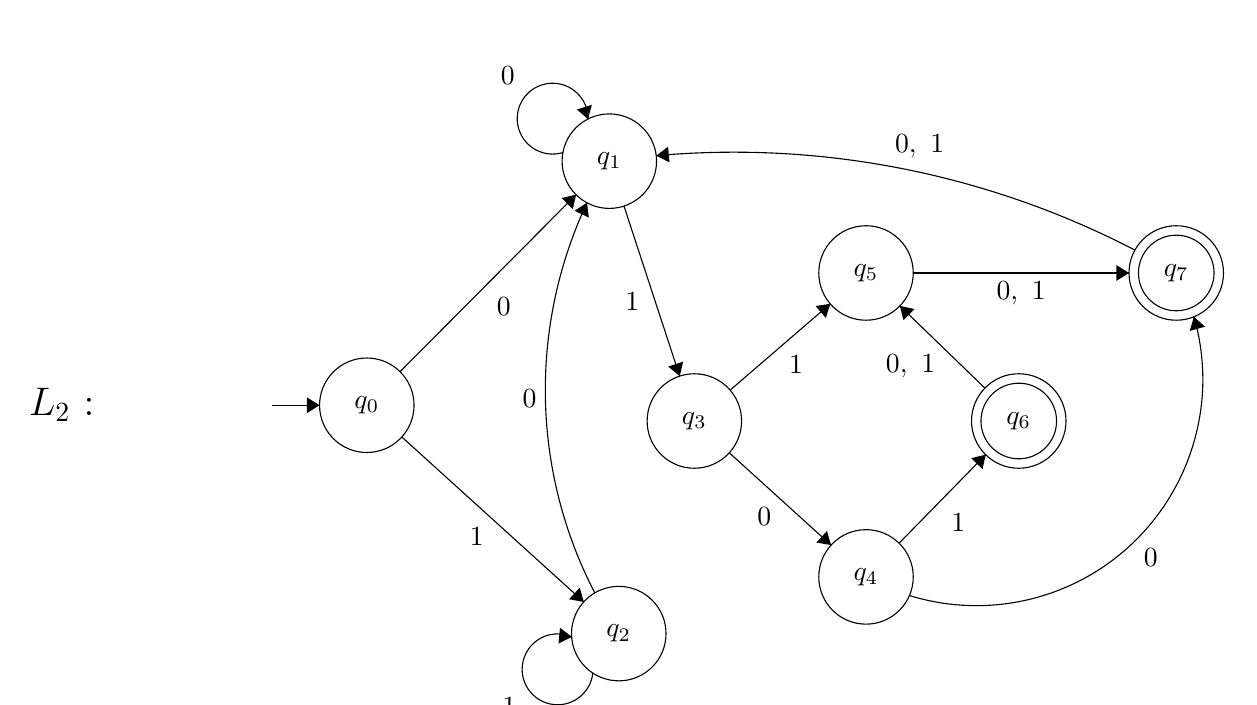
\begin{tikzpicture}[scale=0.2]
\tikzstyle{every node}+=[inner sep=0pt]
\draw [black] (11.5,-31.3) circle (3);
\draw (11.5,-31.3) node {$q_0$};
\draw [black] (26.9,-15.8) circle (3);
\draw (26.9,-15.8) node {$q_1$};
\draw [black] (27.5,-45.8) circle (3);
\draw (27.5,-45.8) node {$q_2$};
\draw [black] (32.3,-32.3) circle (3);
\draw (32.3,-32.3) node {$q_3$};
\draw [black] (43.2,-42.2) circle (3);
\draw (43.2,-42.2) node {$q_4$};
\draw [black] (43.2,-22.9) circle (3);
\draw (43.2,-22.9) node {$q_5$};
\draw [black] (52.9,-32.3) circle (3);
\draw (52.9,-32.3) node {$q_6$};
\draw [black] (52.9,-32.3) circle (2.4);
\draw [black] (62.9,-22.9) circle (3);
\draw (62.9,-22.9) node {$q_7$};
\draw [black] (62.9,-22.9) circle (2.4);
\draw [black] (13.61,-29.17) -- (24.79,-17.93);
\fill [black] (24.79,-17.93) -- (23.87,-18.14) -- (24.58,-18.85);
\draw (19.72,-25.03) node [right] {$0$};
\draw [black] (13.72,-33.31) -- (25.28,-43.79);
\fill [black] (25.28,-43.79) -- (25.02,-42.88) -- (24.35,-43.62);
\draw (18.49,-39.04) node [below] {$1$};
\draw [black] (23.963,-15.25) arc (287.1301:-0.8699:2.25);
\draw (20.92,-10.35) node [left] {$0$};
\fill [black] (25.55,-13.13) -- (25.79,-12.22) -- (24.84,-12.52);
\draw [black] (27.83,-18.65) -- (31.37,-29.45);
\fill [black] (31.37,-29.45) -- (31.59,-28.53) -- (30.64,-28.84);
\draw (28.83,-24.74) node [left] {$1$};
\draw [black] (25.979,-43.216) arc (-152.58244:-205.12604:27.99);
\fill [black] (25.48,-18.44) -- (24.69,-18.95) -- (25.6,-19.38);
\draw (22.31,-30.89) node [left] {$0$};
\draw [black] (25.852,-48.293) arc (-5.74356:-293.74356:2.25);
\draw (21.02,-50.44) node [left] {$1$};
\fill [black] (24.52,-46.01) -- (23.77,-45.43) -- (23.67,-46.43);
\draw [black] (34.52,-34.32) -- (40.98,-40.18);
\fill [black] (40.98,-40.18) -- (40.72,-39.28) -- (40.05,-40.02);
\draw (36.74,-37.74) node [below] {$0$};
\draw [black] (34.57,-30.34) -- (40.93,-24.86);
\fill [black] (40.93,-24.86) -- (40,-25) -- (40.65,-25.76);
\draw (38.76,-28.09) node [below] {$1$};
\draw [black] (45.3,-40.06) -- (50.8,-34.44);
\fill [black] (50.8,-34.44) -- (49.88,-34.66) -- (50.6,-35.36);
\draw (48.58,-38.72) node [right] {$1$};
\draw [black] (64.024,-25.676) arc (16.06498:-107.24023:14.373);
\fill [black] (64.02,-25.68) -- (63.76,-26.58) -- (64.73,-26.31);
\draw (61.29,-40.4) node [below] {$0$};
\draw [black] (46.2,-22.9) -- (59.9,-22.9);
\fill [black] (59.9,-22.9) -- (59.1,-22.4) -- (59.1,-23.4);
\draw (53.05,-23.4) node [below] {$0,\mbox{ }1$};
\draw [black] (50.75,-30.21) -- (45.35,-24.99);
\fill [black] (45.35,-24.99) -- (45.58,-25.9) -- (46.28,-25.19);
\draw (46.03,-28.08) node [below] {$0,\mbox{ }1$};
\draw [black] (29.879,-15.451) arc (95.13277:62.5536:55.229);
\fill [black] (29.88,-15.45) -- (30.72,-15.88) -- (30.63,-14.88);
\draw (46.61,-15.6) node [above] {$0,\mbox{ }1$};
\draw [black] (5.5,-31.3) -- (8.5,-31.3);
\fill [black] (8.5,-31.3) -- (7.7,-30.8) -- (7.7,-31.8);
\draw (-10,-31.3) node [above, anchor=west] {\Large $L_2$ :};
\end{tikzpicture}
\end{flushleft}

% ------------------------------------------------------------
% Question 2
% ------------------------------------------------------------

\newpage
\section{NFAs and DFAs [8 points]}\label{nfatodfa}
Consider the NFA $N = \left(\{q_1, q_2\}, \{0, 1\}, \delta, q_1, \{q_1\}\right)$, with $\delta$ as defined below.
\begin{displaymath}
\begin{array}{|c||c|c|c|}\hline
\delta &       0      &     1     & \emptystring \\\hline\hline
q_1    & \{q_1, q_2\} & \emptyset & \emptyset \\\hline
q_2    & \emptyset    & \{q_1\}   & \{q_1\}   \\\hline
\end{array}
\end{displaymath}
\begin{enumerate}[label=(\roman*)]
\item \textbf{[2 points]} Draw the state diagram for $N$.
\item \textbf{[2 points]} What language does $N$ recognize?
\item \textbf{[3 points]} Let $M_1$ be a DFA recognizing $L(N)$. 
Using the `power set' construction that we saw in class for Theorem 1.39 of the book, 
draw the state diagram for $M_1$ with the corresponding members of \powerset{\set{q_1, q_2}}.
\item \textbf{[1 point]} Let $M_2$ be a DFA recognizing $L(M_1)$ but containing fewer states than $M_1$. 
Draw the state diagram of $M_2$.
\end{enumerate}

\vspace{1em}

\begin{flushleft}
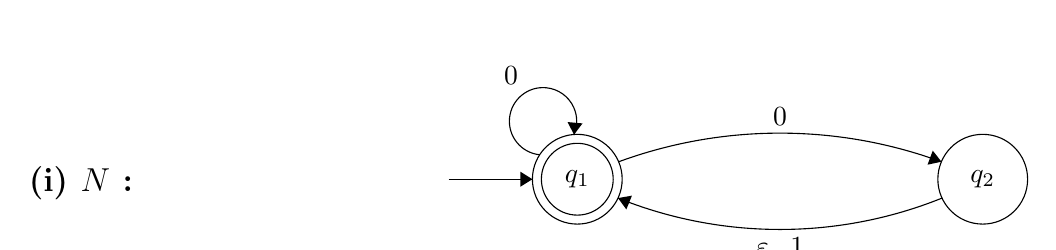
\begin{tikzpicture}[scale=0.19]
\tikzstyle{every node}+=[inner sep=0pt]
\draw [black] (26.7,-30.1) circle (3);
\draw (26.7,-30.1) node {$q_1$};
\draw [black] (26.7,-30.1) circle (2.4);
\draw [black] (53.8,-30.1) circle (3);
\draw (53.8,-30.1) node {$q_2$};
\draw [black] (29.463,-28.934) arc (110.13422:69.86578:31.338);
\fill [black] (51.04,-28.93) -- (50.46,-28.19) -- (50.11,-29.13);
\draw (40.25,-26.52) node [above] {$0$};
\draw [black] (51.08,-31.362) arc (-68.07937:-111.92063:29.009);
\fill [black] (29.42,-31.36) -- (29.98,-32.12) -- (30.35,-31.2);
\draw (40.25,-33.96) node [below] {$\varepsilon,\mbox{ }1$};
\draw [black] (24.198,-28.466) arc (264.57923:-23.42077:2.25);
\draw (22.27,-23.79) node [above] {$0$};
\fill [black] (26.48,-27.12) -- (27.05,-26.37) -- (26.05,-26.28);
\draw [black] (18.1,-30.1) -- (23.7,-30.1);
\fill [black] (23.7,-30.1) -- (22.9,-29.6) -- (22.9,-30.6);

\draw (-10,-30.4) node [above, anchor=west] {\textbf{\large $\text{(i)}$ $N$ :}};
\end{tikzpicture}
\end{flushleft}

\vspace{2em}

\begin{flushleft}
\textbf{\large $\text{(ii)}$ $\text{Language}$ $N$ $\text{recognizes}$:}
\[
L(N) = \{ w \in \{0,1\}^* \mid \text{every 1 in } w \text{ is immediately preceded by a 0} \} \text{ or } (0 \cup 01)^{*}
\]
\end{flushleft}

\vspace{4em}

\begin{center}
\begin{minipage}{0.45\textwidth}
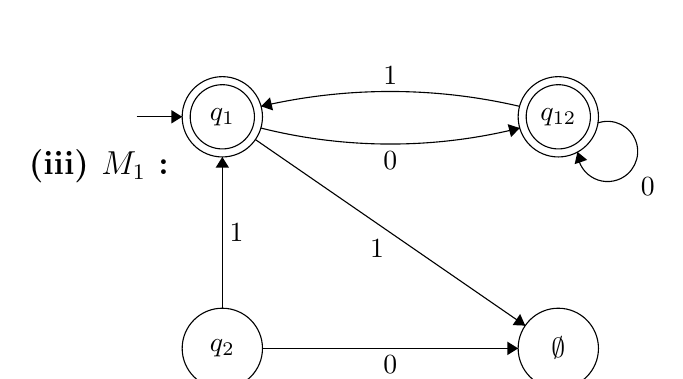
\begin{tikzpicture}[scale=0.17]

   \tikzstyle{every node}+=[inner sep=0pt]
   \draw [black] (19.5,-26.7) circle (3);
   \draw (19.5,-26.7) node {$q_1$};
   \draw [black] (19.5,-26.7) circle (2.4);
   \draw [black] (19.5,-44) circle (3);
   \draw (19.5,-44) node {$q_2$};
   \draw [black] (44.6,-26.7) circle (2.4);
   \draw [black] (44.6,-26.7) circle (3);
   \draw (44.6,-26.7) node {$q_{12}$};
   \draw [black] (44.6,-44) circle (3);
   \draw (44.6,-44) node {$\emptyset$};
   \draw [black] (41.721,-27.54) arc (-75.90446:-104.09554:39.709);
   \fill [black] (41.72,-27.54) -- (40.82,-27.25) -- (41.07,-28.22);
   \draw (32.05,-29.24) node [below] {$0$};
   \draw [black] (19.5,-41) -- (19.5,-29.7);
   \fill [black] (19.5,-29.7) -- (19,-30.5) -- (20,-30.5);
   \draw (20,-35.35) node [right] {$1$};
   \draw [black] (47.553,-27.16) arc (108.87263:-179.12737:2.25);
   \draw (50.72,-31.95) node [right] {$0$};
   \fill [black] (46.03,-29.32) -- (45.82,-30.24) -- (46.76,-29.92);
   \draw [black] (22.395,-25.917) arc (103.1083:76.8917:42.57);
   \fill [black] (22.4,-25.92) -- (23.29,-26.22) -- (23.06,-25.25);
   \draw (32.05,-24.31) node [above] {$1$};
   \draw [black] (21.97,-28.4) -- (42.13,-42.3);
   \fill [black] (42.13,-42.3) -- (41.75,-41.43) -- (41.19,-42.26);
   \draw (31.05,-35.85) node [below] {$1$};
   \draw [black] (22.5,-44) -- (41.6,-44);
   \fill [black] (41.6,-44) -- (40.8,-43.5) -- (40.8,-44.5);
   \draw (32.05,-44.5) node [below] {$0$};
   \draw [black] (13.1,-26.7) -- (16.5,-26.7);
   \fill [black] (16.5,-26.7) -- (15.7,-26.2) -- (15.7,-27.2);

   \draw (5,-30.4) node [above, anchor=west] {\textbf{\large $\text{(iii)}$ $M_1$ :}};

   \end{tikzpicture}
\end{minipage}
\hfill
\begin{minipage}{0.45\textwidth}
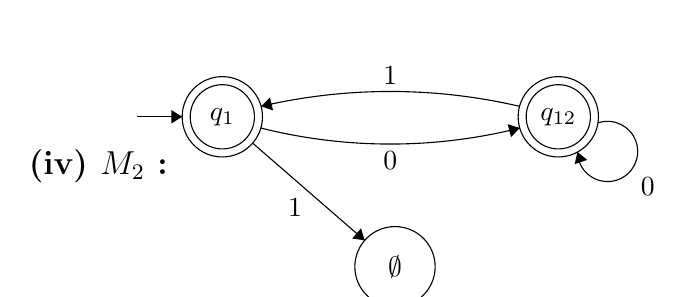
\begin{tikzpicture}[scale=0.17]

   \tikzstyle{every node}+=[inner sep=0pt]
   \draw [black] (19.5,-26.7) circle (3);
   \draw (19.5,-26.7) node {$q_1$};
   \draw [black] (19.5,-26.7) circle (2.4);
   \draw [black] (44.6,-26.7) circle (3);
   \draw (44.6,-26.7) node {$q_{12}$};
   \draw [black] (44.6,-26.7) circle (2.4);
   \draw [black] (32.4,-37.9) circle (3);
   \draw (32.4,-37.9) node {$\emptyset$};
   \draw [black] (41.721,-27.54) arc (-75.90446:-104.09554:39.709);
   \fill [black] (41.72,-27.54) -- (40.82,-27.25) -- (41.07,-28.22);
   \draw (32.05,-29.24) node [below] {$0$};
   \draw [black] (47.553,-27.16) arc (108.87263:-179.12737:2.25);
   \draw (50.72,-31.95) node [right] {$0$};
   \fill [black] (46.03,-29.32) -- (45.82,-30.24) -- (46.76,-29.92);
   \draw [black] (22.395,-25.917) arc (103.1083:76.8917:42.57);
   \fill [black] (22.4,-25.92) -- (23.29,-26.22) -- (23.06,-25.25);
   \draw (32.05,-24.31) node [above] {$1$};
   \draw [black] (21.77,-28.67) -- (30.13,-35.93);
   \fill [black] (30.13,-35.93) -- (29.86,-35.03) -- (29.2,-35.79);
   \draw (24.94,-32.79) node [below] {$1$};
   \draw [black] (13.1,-26.7) -- (16.5,-26.7);
   \fill [black] (16.5,-26.7) -- (15.7,-26.2) -- (15.7,-27.2);

   \draw (5,-30.4) node [above, anchor=west] {\textbf{\large $\text{(iv)}$ $M_2$ :}};

   \end{tikzpicture}
\end{minipage}
\end{center}

% ------------------------------------------------------------
% Question 3
% ------------------------------------------------------------


\newpage
\section{Representation [10 points]}\label{repr}
\begin{enumerate}[label=(\roman*)]
\item \textbf{[1 point]} Argue that if a language can be recognized by a DFA with $k$ states, then it can be recognized by an NFA with $k$ states.
\end{enumerate}
Let $\Sigma = \{0, 1\}$.
Let $\Sigma^n = \underbrace{\Sigma\Sigma\ldots\Sigma}_{n}$.
Consider the regular language $L_k = \Sigma^*1\Sigma^{k-1}$ for some positive integer $k$.
\begin{enumerate}[label=(\roman*)]\setcounter{enumi}{1}
\item \textbf{[2 points]} Show that $L_k$ can be recognized by an NFA with $k+1$ states.
\item \textbf{[4 points]} Prove that any DFA recognizing $L_k$ must have at least $2^k$ states.
\item \textbf{[2 points]} What does part (iii) of this question tell you about Theorem 1.39 from the book?
\item \textbf{[1 point]} What do parts (i), (ii), and (iii) of this question tell you about DFAs as compared to NFAs? 
\end{enumerate}

\vspace{.7em}


\noindent\textbf{Answer to (i):}

Every DFA is, by definition, also an NFA. This is because an NFA (Nondeterministic Finite Automaton) is a generalization of a DFA (Deterministic Finite Automaton).

\vspace{.3em}

A DFA is simply a special case of an NFA where:
\begin{enumerate}
\item For each state and each input symbol, there is exactly one transition (no nondeterminism)
\item There are no $\varepsilon$-transitions (empty string transitions)
\end{enumerate}

Therefore, any DFA with $k$ states can be viewed directly as an NFA with $k$ states that happens to be deterministic. The transition function, start state, and accepting states remain the same. No conversion is needed, the DFA already satisfies all the requirements of being an NFA.

\vspace{1em}

\noindent\textbf{Answer to (ii):}

We can construct an NFA with $k + 1$ states as follows:

\vspace{.2em}

\textbf{States:} $Q = \{q_0, q_1, q_2, \ldots, q_k\}$

\vspace{.2em}

\textbf{Construction:}
\begin{itemize}
\item $q_0$ is the start state
\item $q_k$ is the only accepting state
\item From $q_0$: 
  \begin{itemize}
  \item On input $0$ or $1$: stay in $q_0$ (loop)
  \item On input $1$: \emph{nondeterministically} transition to $q_1$ (this is the ``guess'' that we've seen the $1$ that is $k$ positions from the end)
  \end{itemize}
\item From $q_i$ (for $i = 1, 2, \ldots, k-1$):
  \begin{itemize}
  \item On input $0$ or $1$: transition to $q_{i+1}$
  \end{itemize}
\item $q_k$ is the accepting state (reached after reading exactly $k-1$ more symbols after the crucial $1$)
\end{itemize}

\textbf{How it works:} The NFA uses nondeterminism to ``guess'' when it sees the $1$ that is exactly $k$ positions from the end. It stays in $q_0$ reading arbitrary input until it nondeterministically decides to move to $q_1$ upon seeing a $1$. Then it must read exactly $k-1$ more characters (states $q_1 \to q_2 \to \cdots \to q_k$). If the string ends exactly when reaching $q_k$, it accepts.

\textbf{State count:} This NFA has exactly $k + 1$ states $(q_0, q_1, \ldots, q_k)$.

\newpage


\noindent\textbf{Answer to (iii):}

\textbf{Proof by contradiction:}

Assume, for the sake of contradiction, that there exists a DFA $M$ that recognizes $L_k$ and has fewer than $2^k$ states.

Consider all possible strings of length $k$ over $\Sigma = \{0, 1\}$. There are exactly $2^k$ such strings. Let's call this set $S = \Sigma^k = \{x_1, x_2, \ldots, x_{2^k}\}$.

Since $M$ has fewer than $2^k$ states, and we are reading $2^k$ different strings, by the \textbf{Pigeonhole Principle}, at least two distinct strings from $S$ must lead to the same state in $M$.

Let's call these two strings $x$ and $y$ where $x \neq y$, and both are in $\Sigma^k$. Write:
\begin{itemize}
\item $x = x_1x_2\cdots x_k$
\item $y = y_1y_2\cdots y_k$
\end{itemize}

Since $x \neq y$, there must exist some position $i$ where $1 \leq i \leq k$ and $x_i \neq y_i$.

Without loss of generality, assume $x_i = 1$ and $y_i = 0$.

Now consider the string $z$ consisting of any $(k-i)$ symbols from $\Sigma$. In other words, $z \in \Sigma^{k-i}$.

Observe:
\begin{itemize}
\item In $xz = x_1x_2\cdots x_kz$, the $k$-th character from the end is $x_i = 1$, so $xz \in L_k$
\item In $yz = y_1y_2\cdots y_kz$, the $k$-th character from the end is $y_i = 0$, so $yz \notin L_k$
\end{itemize}

Since $x$ and $y$ lead to the same state in $M$, and $M$ is deterministic, reading the same suffix $z$ from that state must lead to the same final state. Therefore:
\begin{itemize}
\item Either both $xz$ and $yz$ are accepted by $M$
\item Or both $xz$ and $yz$ are rejected by $M$
\end{itemize}

But we just showed that $xz \in L_k$ (should be accepted) and $yz \notin L_k$ (should be rejected).

This is a \textbf{contradiction.} The DFA $M$ cannot correctly recognize $L_k$ if it accepts both or rejects both. 

Therefore, our assumption must be false, and any DFA recognizing $L_k$ must have \textbf{at least $2^k$ states}. 

\vspace{1em}

\newpage

\noindent\textbf{Answer to (iv):}

Theorem 1.39 (the NFA to DFA conversion theorem) states that for every NFA, there exists an equivalent DFA. The standard subset construction algorithm can convert an NFA with $n$ states to a DFA with at most $2^n$ states.

Part (iii) demonstrates that this exponential blow-up is not just a theoretical upper bound, but can actually occur in practice:

\begin{itemize}
\item The NFA for $L_k$ has $k + 1$ states (from part ii)
\item The minimum DFA for $L_k$ has $2^k$ states (from part iii)
\end{itemize}

This shows that:
\begin{enumerate}
\item The conversion from NFA to DFA can indeed require exponentially many states
\item The $2^n$ upper bound in the subset construction is tight, there exist languages where the exponential blow-up actually happens
\item While every NFA can be converted to a DFA (proving NFA and DFA have the same expressive power), the size cost can be exponential
\end{enumerate}

\vspace{1em}

\noindent\textbf{Answer to (v):}

Combining parts (i), (ii), and (iii):

\textbf{Expressive power:} DFAs and NFAs are equivalent in terms of the languages they can recognize (both recognize exactly the regular languages).

\textbf{Succinctness:} NFAs can be \emph{exponentially more succinct} than DFAs. For the language $L_k$:
\begin{itemize}
\item NFA requires only $k + 1$ states
\item DFA requires $2^k$ states
\end{itemize}

This is an exponential gap $(2^k$ vs. $k+1)$.

\textbf{Key insight:} While NFAs and DFAs recognize the same class of languages, NFAs can represent some languages much more efficiently. Nondeterminism allows for more compact representations at the cost of more complex acceptance semantics (multiple possible computation paths).

% ------------------------------------------------------------
% Question 4
% ------------------------------------------------------------

\newpage
\section{Regular Expressions [4 points; 2 points each]}
Let $\Sigma = \set{0, 1}$. Give regular expressions for the following languages.
\begin{enumerate}[label=(\roman*)]
\item $L_1 = \set{w \mid \mbox{every even position of $w = w_1w_2\ldots w_n$ has a 0}}$.
\item $L_2 = \set{w \mid \mbox{$w$ interpreted as a binary number is divisible by 2 (or 10 in binary)}}$.
\end{enumerate}
Note that $\emptystring\in L_1$, whereas $\emptystring\not\in L_2$.

\vspace{1em}

\noindent\textbf{Answer to (i):}

\textbf{Understanding:} Positions are numbered starting from 1. Even positions (2, 4, 6, ...) must be 0. Odd positions (1, 3, 5, ...) can be 0 or 1.

\textbf{Pattern:} The repeating pattern is $(0 \cup 1)0$ (any symbol followed by 0). This pattern repeats zero or more times, and we may have one final odd-positioned character (or none for the empty string).

\textbf{Regular expression:} 
\[
((0 \cup 1)0)^*(\varepsilon \cup 0 \cup 1)
\]

\textbf{Verification:}
\begin{itemize}
\item $\varepsilon$: accepted (no even positions) \cmark
\item $0, 1$: accepted (only odd position 1) \cmark
\item $00, 10$: accepted (position 2 is 0) \cmark
\item $01, 11$: rejected (position 2 is 1) \xmark
\item $1001$: accepted (positions 2 and 4 are both 0) \cmark
\item $1011$: rejected (position 4 is 1) \xmark
\end{itemize}

\vspace{1em}

\noindent\textbf{Answer to (ii):}

\textbf{Key insight:} A binary number is divisible by 2 if and only if it ends in 0 (just like decimal numbers divisible by 10 end in 0).

\textbf{Regular expression:}
\[
(0 \cup 1)^*0
\]

This accepts any string that ends in 0.

\textbf{Verification:}
\begin{itemize}
\item $0 = 0_{10}$: divisible by 2 \cmark
\item $10 = 2_{10}$: divisible by 2 \cmark
\item $100 = 4_{10}$: divisible by 2 \cmark
\item $110 = 6_{10}$: divisible by 2 \cmark
\item $1 = 1_{10}$: not divisible by 2 \xmark
\item $11 = 3_{10}$: not divisible by 2 \xmark
\item $\varepsilon$: not accepted \cmark
\end{itemize}

% ------------------------------------------------------------
% Question 5
% ------------------------------------------------------------

\newpage
\section{DFAs to Regular Expressions [6 points]}\label{conversion}
Convert the following DFA to a regular expression. 
\begin{center}
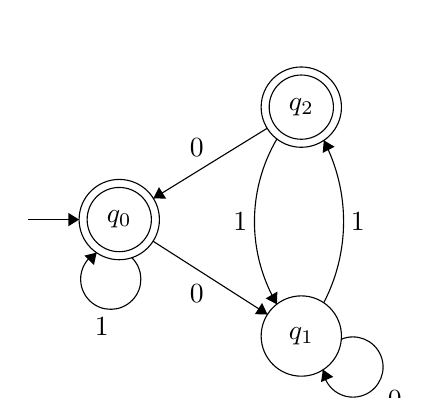
\begin{tikzpicture}[scale=0.17]
\tikzstyle{every node}+=[inner sep=0pt]
\draw [black] (31.8,-30.2) circle (3);
\draw (31.8,-30.2) node {$q_0$};
\draw [black] (31.8,-30.2) circle (2.4);
\draw [black] (45.4,-38.9) circle (3);
\draw (45.4,-38.9) node {$q_1$};
\draw [black] (45.4,-21.8) circle (3);
\draw (45.4,-21.8) node {$q_2$};
\draw [black] (45.4,-21.8) circle (2.4);
\draw [black] (42.85,-23.38) -- (34.35,-28.62);
\fill [black] (34.35,-28.62) -- (35.3,-28.63) -- (34.77,-27.78);
\draw (37.6,-25.5) node [above] {$0$};
\draw [black] (34.33,-31.82) -- (42.87,-37.28);
\fill [black] (42.87,-37.28) -- (42.47,-36.43) -- (41.93,-37.27);
\draw (37.6,-35.05) node [below] {$0$};
\draw [black] (47.075,-24.281) arc (27.48941:-27.48941:13.148);
\fill [black] (47.08,-24.28) -- (47,-25.22) -- (47.89,-24.76);
\draw (49.06,-30.35) node [right] {$1$};
\draw [black] (43.579,-36.525) arc (-149.57195:-210.42805:12.193);
\fill [black] (43.58,-36.53) -- (43.61,-35.58) -- (42.74,-36.09);
\draw (41.4,-30.35) node [left] {$1$};
\draw [black] (48.378,-39.145) arc (113.03624:-174.96376:2.25);
\draw (51.83,-43.64) node [right] {$0$};
\fill [black] (47.02,-41.41) -- (46.87,-42.34) -- (47.79,-41.95);
\draw [black] (32.73,-33.04) arc (45.8699:-242.1301:2.25);
\draw (30.5,-37.48) node [below] {$1$};
\fill [black] (30.11,-32.67) -- (29.2,-32.89) -- (29.91,-33.59);
\draw [black] (25,-30.2) -- (28.8,-30.2);
\fill [black] (28.8,-30.2) -- (28,-29.7) -- (28,-30.7);
\end{tikzpicture}
\end{center}

Do so by starting from the equivalent GNFA, then remove the state $q_1$, then the state $q_2$ and finally the state $q_0$.

\vspace{1em}

\subsection*{Solution}

\textbf{Step 0: Convert DFA to GNFA}

Add new start state $q_{start}$ and new accept state $q_{accept}$:
\begin{itemize}
\item $q_{start} \xrightarrow{\varepsilon} q_0$
\item $q_0 \xrightarrow{\varepsilon} q_{accept}$ (since $q_0$ is accepting)
\item $q_2 \xrightarrow{\varepsilon} q_{accept}$ (since $q_2$ is accepting)
\end{itemize}

All other transitions remain with their labels.

\vspace{1em}

\textbf{Step 1: Remove $q_1$}

When removing a state $q$, for each pair of states $p$ and $r$ (where $p \neq q$ and $r \neq q$), replace the path $p \to q \to r$ with:
\[
R_{new}(p,r) = R(p,r) \cup R(p,q) \cdot R(q,q)^* \cdot R(q,r)
\]

\textbf{Paths through $q_1$:}
\begin{enumerate}
\item $q_0$ to $q_2$ through $q_1$: $q_0 \xrightarrow{0} q_1 \xrightarrow{0^*} q_1 \xrightarrow{1} q_2$

New edge: $q_0 \xrightarrow{00^*1} q_2$

\item $q_2$ to $q_2$ through $q_1$: $q_2 \xrightarrow{1} q_1 \xrightarrow{0^*} q_1 \xrightarrow{1} q_2$

New edge: $q_2 \xrightarrow{10^*1} q_2$ (self-loop)
\end{enumerate}

\textbf{After removing $q_1$:}
\begin{itemize}
\item $q_0 \xrightarrow{1} q_0$ (self-loop)
\item $q_0 \xrightarrow{00^*1} q_2$
\item $q_0 \xrightarrow{\varepsilon} q_{accept}$
\item $q_2 \xrightarrow{0} q_0$
\item $q_2 \xrightarrow{10^*1} q_2$ (self-loop)
\item $q_2 \xrightarrow{\varepsilon} q_{accept}$
\end{itemize}

\vspace{1em}

\textbf{Step 2: Remove $q_2$}

\textbf{Paths through $q_2$:}
\begin{enumerate}
\item $q_0$ to $q_0$ through $q_2$: $q_0 \xrightarrow{00^*1} q_2 \xrightarrow{(10^*1)^*} q_2 \xrightarrow{0} q_0$

New edge: $q_0 \xrightarrow{00^*1(10^*1)^*0} q_0$

\item $q_0$ to $q_{accept}$ through $q_2$: $q_0 \xrightarrow{00^*1} q_2 \xrightarrow{(10^*1)^*} q_2 \xrightarrow{\varepsilon} q_{accept}$

New edge: $q_0 \xrightarrow{00^*1(10^*1)^*} q_{accept}$
\end{enumerate}

\textbf{After removing $q_2$:}
\begin{itemize}
\item $q_0 \xrightarrow{1 \cup 00^*1(10^*1)^*0} q_0$ (combined self-loops)
\item $q_0 \xrightarrow{\varepsilon \cup 00^*1(10^*1)^*} q_{accept}$
\end{itemize}

\vspace{1em}

\textbf{Step 3: Remove $q_0$}

Apply the formula:
\[
R(q_{start}, q_{accept}) = R(q_{start}, q_0) \cdot R(q_0, q_0)^* \cdot R(q_0, q_{accept})
\]

Substituting:
\[
= \varepsilon \cdot (1 \cup 00^*1(10^*1)^*0)^* \cdot (\varepsilon \cup 00^*1(10^*1)^*)
\]

Since $\varepsilon$ is the identity for concatenation ($\varepsilon \cdot R = R$):
\[
= (1 \cup 00^*1(10^*1)^*0)^* \cdot (\varepsilon \cup 00^*1(10^*1)^*)
\]

\vspace{1em}

\textbf{Final Regular Expression:}
\[
\boxed{(1 \cup 00^*1(10^*1)^*0)^*(\varepsilon \cup 00^*1(10^*1)^*)}
\]

\newpage

% Diagram representation of the conversion from DFA to GNFA

\begin{center}
   \textbf{\large \text{Covnerting the DFA to a GNFA - diagrams:}}
\end{center}

\begin{center}
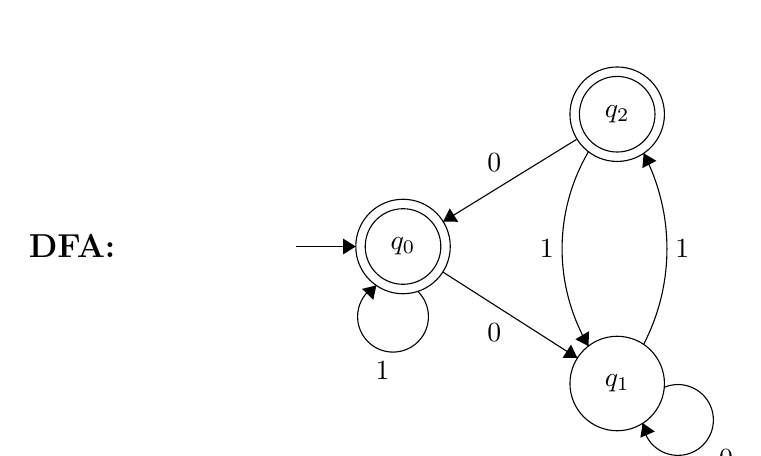
\begin{tikzpicture}[scale=0.2]
\tikzstyle{every node}+=[inner sep=0pt]
\draw [black] (31.8,-30.2) circle (3);
\draw (31.8,-30.2) node {$q_0$};
\draw [black] (31.8,-30.2) circle (2.4);
\draw [black] (45.4,-38.9) circle (3);
\draw (45.4,-38.9) node {$q_1$};
\draw [black] (45.4,-21.8) circle (3);
\draw (45.4,-21.8) node {$q_2$};
\draw [black] (45.4,-21.8) circle (2.4);
\draw [black] (42.85,-23.38) -- (34.35,-28.62);
\fill [black] (34.35,-28.62) -- (35.3,-28.63) -- (34.77,-27.78);
\draw (37.6,-25.5) node [above] {$0$};
\draw [black] (34.33,-31.82) -- (42.87,-37.28);
\fill [black] (42.87,-37.28) -- (42.47,-36.43) -- (41.93,-37.27);
\draw (37.6,-35.05) node [below] {$0$};
\draw [black] (47.075,-24.281) arc (27.48941:-27.48941:13.148);
\fill [black] (47.08,-24.28) -- (47,-25.22) -- (47.89,-24.76);
\draw (49.06,-30.35) node [right] {$1$};
\draw [black] (43.579,-36.525) arc (-149.57195:-210.42805:12.193);
\fill [black] (43.58,-36.53) -- (43.61,-35.58) -- (42.74,-36.09);
\draw (41.4,-30.35) node [left] {$1$};
\draw [black] (48.378,-39.145) arc (113.03624:-174.96376:2.25);
\draw (51.83,-43.64) node [right] {$0$};
\fill [black] (47.02,-41.41) -- (46.87,-42.34) -- (47.79,-41.95);
\draw [black] (32.73,-33.04) arc (45.8699:-242.1301:2.25);
\draw (30.5,-37.48) node [below] {$1$};
\fill [black] (30.11,-32.67) -- (29.2,-32.89) -- (29.91,-33.59);
\draw [black] (25,-30.2) -- (28.8,-30.2);
\fill [black] (28.8,-30.2) -- (28,-29.7) -- (28,-30.7);
\draw (8,-30.2) node [above, anchor=west] {\textbf{\large \text{DFA:}}};
\end{tikzpicture}
\end{center}

\vspace{2em}
\begin{center}
    \noindent\rule{0.7\textwidth}{0.4pt}
\end{center}
\vspace{2em}

% removing q_1
\begin{flushleft}
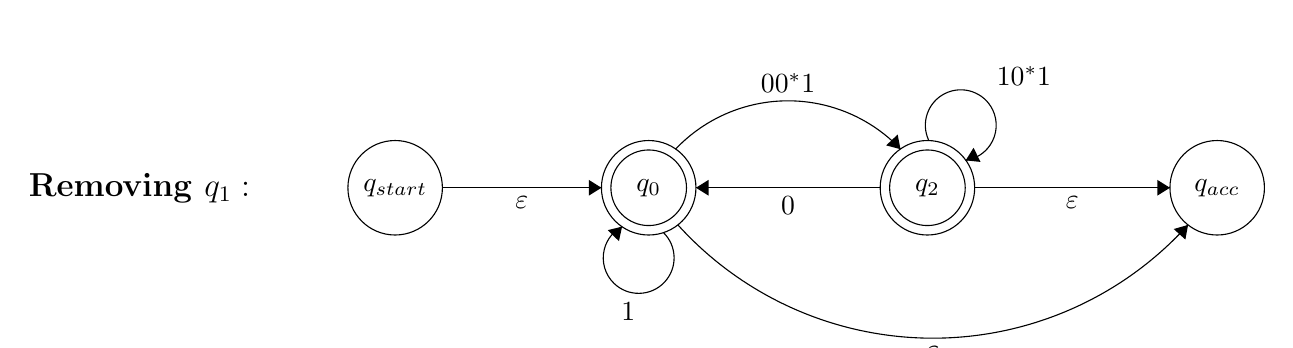
\begin{tikzpicture}[scale=0.2]
\tikzstyle{every node}+=[inner sep=0pt]
\draw [black] (29.4,-29.3) circle (3);
\draw (29.4,-29.3) node {$q_0$};
\draw [black] (29.4,-29.3) circle (2.4);
\draw [black] (47.1,-29.3) circle (3);
\draw (47.1,-29.3) node {$q_2$};
\draw [black] (47.1,-29.3) circle (2.4);
\draw [black] (13.3,-29.3) circle (3);
\draw (13.3,-29.3) node {$q_{start}$};
\draw [black] (65.5,-29.3) circle (3);
\draw (65.5,-29.3) node {$q_{acc}$};
\draw [black] (44.1,-29.3) -- (32.4,-29.3);
\fill [black] (32.4,-29.3) -- (33.2,-29.8) -- (33.2,-28.8);
\draw (38.25,-29.8) node [below] {$0$};
\draw [black] (30.33,-32.14) arc (45.8699:-242.1301:2.25);
\draw (28.1,-36.58) node [below] {$1$};
\fill [black] (27.71,-31.77) -- (26.8,-31.99) -- (27.51,-32.69);
\draw [black] (16.3,-29.3) -- (26.4,-29.3);
\fill [black] (26.4,-29.3) -- (25.6,-28.8) -- (25.6,-29.8);
\draw (21.35,-29.8) node [below] {$\varepsilon$};
\draw [black] (63.648,-31.657) arc (-42.09909:-137.90091:21.83);
\fill [black] (63.65,-31.66) -- (62.74,-31.92) -- (63.48,-32.59);
\draw (47.45,-39.35) node [below] {$\varepsilon$};
\draw [black] (50.1,-29.3) -- (62.5,-29.3);
\fill [black] (62.5,-29.3) -- (61.7,-28.8) -- (61.7,-29.8);
\draw (56.3,-29.8) node [below] {$\varepsilon$};
\draw [black] (31.106,-26.846) arc (136.47491:43.52509:9.853);
\fill [black] (45.39,-26.85) -- (45.21,-25.92) -- (44.48,-26.61);
\draw (38.25,-23.28) node [above] {$00^*1$};
\draw [black] (47.194,-26.313) arc (205.92751:-82.07249:2.25);
\draw (53.23,-22.84) node [above] {$10^*1$};
\fill [black] (49.53,-27.56) -- (50.47,-27.66) -- (50.03,-26.76);
\draw (-10,-29.3) node [above, anchor=west] {\textbf{\large \text{Removing} $q_1:$}};
\end{tikzpicture}
\end{flushleft}

\vspace{3em}

% removing q_2
\begin{flushleft}
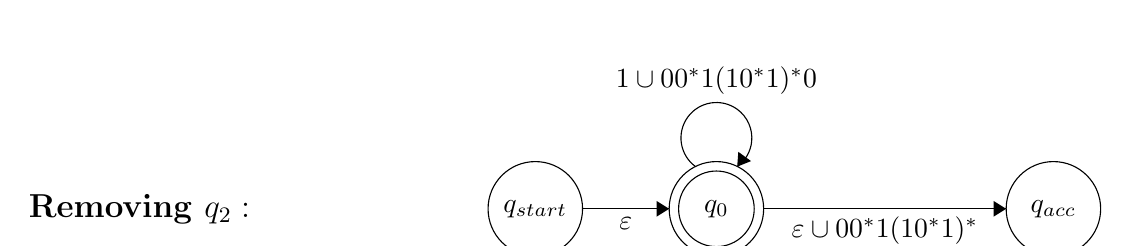
\begin{tikzpicture}[scale=0.2]
\tikzstyle{every node}+=[inner sep=0pt]
\draw [black] (39.7,-29.3) circle (3);
\draw (39.7,-29.3) node {$q_0$};
\draw [black] (39.7,-29.3) circle (2.4);
\draw [black] (28.2,-29.3) circle (3);
\draw (28.2,-29.3) node {$q_{start}$};
\draw [black] (61.1,-29.3) circle (3);
\draw (61.1,-29.3) node {$q_{acc}$};
\draw [black] (31.2,-29.3) -- (36.7,-29.3);
\fill [black] (36.7,-29.3) -- (35.9,-28.8) -- (35.9,-29.8);
\draw (33.95,-29.8) node [below] {$\varepsilon$};
\draw [black] (42.7,-29.3) -- (58.1,-29.3);
\fill [black] (58.1,-29.3) -- (57.3,-28.8) -- (57.3,-29.8);
\draw (50.4,-29.8) node [below] {$\varepsilon\cup00^*1(10^*1)^*$};
\draw [black] (38.377,-26.62) arc (234:-54:2.25);
\draw (39.7,-22.05) node [above] {$1\cup00^*1(10^*1)^*0$};
\fill [black] (41.02,-26.62) -- (41.9,-26.27) -- (41.09,-25.68);
\draw (-4,-29.3) node [above, anchor=west] {\textbf{\large \text{Removing} $q_2:$}};
\end{tikzpicture}
\end{flushleft}

\vspace{3em}

% removing q_0
\begin{flushleft}
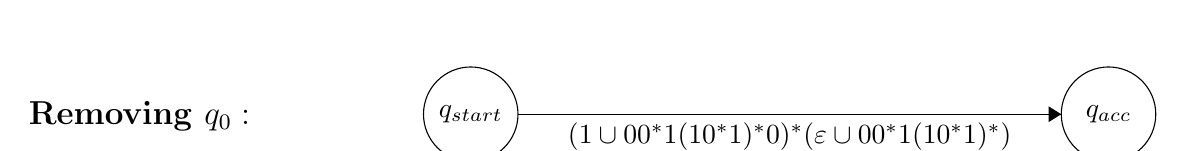
\begin{tikzpicture}[scale=0.2]
\tikzstyle{every node}+=[inner sep=0pt]
\draw [black] (25.1,-29.2) circle (3);
\draw (25.1,-29.2) node {$q_{start}$};
\draw [black] (65.6,-29.2) circle (3);
\draw (65.6,-29.2) node {$q_{acc}$};
\draw [black] (28.1,-29.2) -- (62.6,-29.2);
\fill [black] (62.6,-29.2) -- (61.8,-28.7) -- (61.8,-29.7);
\draw (45.35,-29.7) node [below] {$(1\cup00^*1(10^*1)^*0)^*(\varepsilon\cup00^*1(10^*1)^*)$};
\draw (-3,-29.3) node [above, anchor=west] {\textbf{\large \text{Removing} $q_0:$}};
\end{tikzpicture}
\end{flushleft}


% ------------------------------------------------------------
% Question 6
% ------------------------------------------------------------


\newpage
\section{Non Regular Languages [8 points]}\label{non-regular}
Use the Pumping Lemma to prove that the following languages are \textbf{not} regular.
\begin{enumerate}[label=(\roman*)]
\item $L_1 = \set{www \mid w\in\Sigma^*}$, $\Sigma = \set{0, 1}$.
\item $L_2 = \set{1^{2^n} \mid n\ge 1}$, $\Sigma = \set{1}$.
\end{enumerate}

\vspace{1em}

\subsection*{Solution}

\noindent\textbf{(i) Proof for $L_1 = \set{www \mid w\in\Sigma^*}$}

\textbf{Proof by contradiction:}

Assume $L_1$ is regular. Then by the Pumping Lemma, there exists a pumping length $p$.

\textbf{Choose a string:} Let $w \in \Sigma^*$ be any string with $|w| = p$. Consider $s = www$.

Then $s \in L_1$ and $|s| = 3p \geq p$.

By the Pumping Lemma, we can write $s = xyz$ where:
\begin{itemize}
\item $|y| > 0$
\item $|xy| \leq p$
\item For all $i \geq 0$, $xy^iz \in L_1$
\end{itemize}

\textbf{Analysis of the split:}

Since $s = www$ with $|w| = p$, we can view the string as three consecutive copies of $w$:
\[
s = \underbrace{w}_{\text{1st copy}} \hspace{0.5em} \underbrace{w}_{\text{2nd copy}} \hspace{0.5em} \underbrace{w}_{\text{3rd copy}}
\]

The constraint $|xy| \leq p$ means that $xy$ is entirely contained within the first copy of $w$ (since the first $w$ has length $p$).

Since $xy$ lies within the first $w$:
\begin{itemize}
\item $x$ corresponds to some prefix of $w$ (possibly empty)
\item $y$ corresponds to the next part of $w$ (non-empty, since $|y| > 0$)
\item $z$ consists of the remainder of the first $w$ (if $|xy| < p$) plus the entire second and third copies of $w$, OR just the second and third copies of $w$ (if $|xy| = p$)
\end{itemize}

\textbf{Pumping to get a contradiction:}

Consider $i = 2$ (pump once). Then:
\[
xy^2z = xyyz
\]

Since $xy$ lies entirely within the first copy of $w$, pumping $y$ adds extra characters only to the first copy. The second and third copies of $w$ remain completely unchanged.

For $xy^2z$ to be in $L_1$, it must equal $w'w'w'$ for some string $w' \in \Sigma^*$ (three identical copies).

However:
\begin{itemize}
\item The first part of $xy^2z$ has been lengthened by $|y|$ characters (since we added an extra copy of $y$)
\item The second and third parts remain as the original $w$
\end{itemize}

Since $|y| > 0$, the first part is now different from the second and third parts. Therefore, $xy^2z$ cannot be written as three identical copies.

Therefore, $xy^2z \notin L_1$.

This is a \textbf{contradiction.} Therefore, $L_1$ is not regular. $\square$

\vspace{2em}

\noindent\textbf{(ii) Proof for $L_2 = \set{1^{2^n} \mid n\ge 1}$}

\textbf{Proof by contradiction:}

Assume $L_2$ is regular. Then by the Pumping Lemma, there exists a pumping length $p$.

\textbf{Choose a string:} Let $s = 1^{2^p}$.

Then $s \in L_2$ and $|s| = 2^p \geq p$.

By the Pumping Lemma, we can write $s = xyz$ where:
\begin{itemize}
\item $|y| > 0$
\item $|xy| \leq p$
\item For all $i \geq 0$, $xy^iz \in L_2$
\end{itemize}

\textbf{Analysis of the constraints:}

From the Pumping Lemma conditions:
\begin{itemize}
\item Since $|xy| \leq p$, we have $|y| \leq p$
\item Since $|y| > 0$, we know $y$ is non-empty
\end{itemize}

\textbf{Pumping to get a contradiction:}

Consider $i = 2$ (pump once). Compare the original string $xyz$ with the pumped string $xy^2z$.

The original string has length: $|xyz| = 2^p$

The pumped string has length: $|xy^2z| = |xyz| + |y| = 2^p + |y|$

Since $0 < |y| \leq p$, we can establish bounds on the pumped length:
\begin{itemize}
\item \textbf{Lower bound:} $|xy^2z| = 2^p + |y| > 2^p$ (since $|y| > 0$)
\item \textbf{Upper bound:} $|xy^2z| = 2^p + |y| \leq 2^p + p$
\end{itemize}

Now, for $p \geq 1$, we have $p < 2^p$ (exponential growth), which means:
\[
2^p + p < 2^p + 2^p = 2 \cdot 2^p = 2^{p+1}
\]

Combining these inequalities:
\[
2^p < |xy^2z| \leq 2^p + p < 2^{p+1}
\]

\textbf{The contradiction:}

For $xy^2z$ to be in $L_2$, its length must be a power of 2. However, we've shown that:
\[
2^p < |xy^2z| < 2^{p+1}
\]

This means the length of $xy^2z$ is strictly between two consecutive powers of 2. Since there are no powers of 2 between $2^p$ and $2^{p+1}$, we have $xy^2z \notin L_2$.

This contradicts the Pumping Lemma, which states that $xy^2z$ must be in $L_2$.

Therefore, our assumption is false, and $L_2$ is not regular. $\square$

\end{document}
